% =====================================================================
%  chunks/ch03b.tex —— 原书 p.47–56（PDF 54–63）
%  第 3 章 §2 同调群与上同调群、Poincaré 对偶
% =====================================================================
% [原文 p.47]
（因此，两个单形的乘积虽不是单形，却容易三角剖分——见图 3.5。）

\section{同调群与上同调群。Poincaré 对偶}
\takeaway{本节把单纯复形的链、闭链、边缘与同调群严格地定义：先由单形的代数边缘 (2.1) 导出边缘算子与链复形 (2.2)，再取 $\Ker\partial/\Image\partial$ 得同调群 (2.3)；随后用 $\otimes$、$\Hom$ 与万有系数公式把同调与上同调、整系数与任意系数域联系起来，最后给出紧致可定向流形的 Poincaré 对偶。}

现在转向单纯复形的同调群与上同调群的定义。任意单形 $\sigma^n=(\alpha_0,\dots,\alpha_n)$ 的\emph{代数边缘}，定义为它的 $n-1$ 维面如下形式的线性组合：
\begin{equation}
  \partial\sigma^n=\sum_{i=0}^{n}(-1)^i\sigma_i^{n-1}, \tag{2.1}
\end{equation}
其中 $\sigma_i^{n-1}=(\alpha_0,\dots,\widehat{\alpha_i},\dots,\alpha_n)$，$\widehat{\alpha_i}$ 上的帽子表示略去 $\alpha_i$。注意 $\partial\circ\partial=0$。对任意复形 $K$，$K$ 的 $n$ 维\emph{整链群} $C_n(K)$ 是由 $K$ 的 $n$-单形的全体有限整系数线性组合构成的自由交换群：
\[
  c\in C_n(K),\qquad c=\sum_{\alpha}\lambda_{\alpha}\sigma_{\alpha}^{n},\quad \sigma_{\alpha}^{n}\in K;
\]
这里 $\alpha$ 对 $K$ 的 $n$-单形取指标，系数 $\lambda_{\alpha}$ 是整数。由单形代数边缘的定义式 (2.1)，得到 $K$ 的整 $n$-链上的\emph{边缘算子} $\partial$：
\[
  \partial: C_n(K)\to C_{n-1}(K),\qquad
  \partial\Bigl(\sum_{\alpha}\lambda_{\alpha}\sigma_{\alpha}^{n}\Bigr)
  =\sum_{\alpha}\lambda_{\alpha}\,(\partial\sigma_{\alpha}^{n}),
\]
进而得到链复形 $C_*(K)$：
\begin{equation}
  \cdots\xrightarrow{\partial}C_n(K)\xrightarrow{\partial}C_{n-1}(K)
  \xrightarrow{\partial}C_{n-2}(K)\xrightarrow{\partial}\cdots
  \xrightarrow{\partial}C_0(K)\xrightarrow{\partial}0, \tag{2.2}
\end{equation}
其中 $\partial\circ\partial=0$。现在对每个 $n\ge 0$，定义 $K$ 的 $n$ 维\emph{整同调群}为
\begin{equation}
  H_n(K;\Z)=\Ker\partial/\Image\partial, \tag{2.3}
\end{equation}
并注意这一写法有意义，即 $\Ker\partial\supset\Image\partial$，因为 $\partial\circ\partial=0$。子群 $\Ker\partial\subset C_n(K)$ 的元素称为 $K$ 的\emph{闭链}，子群 $\Image\partial\subset C_n(K)$ 的元素称为\emph{边缘}。

从任意一对（加法写法的）交换群 $G_1,G_2$ 出发构造 $G_1\otimes G_2$ 与 $\Hom(G_1,G_2)$ 的运算，对我们很重要；它们定义如下：

1. 交换群 $G_1\otimes G_2$ 这样得到：取形如 $g_1\otimes g_2$（$g_1\in G_1$，$g_2\in G_2$）的表达式的一切有限形式和构成的群，再商去双线性关系：
% [原文 p.48]
\begin{align}
  (g_1'+g_1'')\otimes g_2 &= g_1'\otimes g_2+g_1''\otimes g_2,\notag\\
  g_1\otimes(g_2'+g_2'') &= g_1\otimes g_2'+g_1\otimes g_2''. \tag{2.4}
\end{align}
所得群 $G_1\otimes G_2$ 称为 $G_1$ 与 $G_2$ 的\emph{张量积}。

2. 交换群 $\Hom(G_1,G_2)$ 的元素，是从交换群 $G_1$ 到交换群 $G_2$ 的同态 $h:G_1\to G_2$；两个这样的同态按自然方式相加：
\begin{equation}
  (h_1+h_2)(g)=h_1(g)+h_2(g). \tag{2.5}
\end{equation}

当 $G_2$ 是某个域的加法群时，把 $\Hom(G_1,G_2)$ 记作 $G_1^*$。（比较向量空间 $V$ 的对偶空间记号 $V^*$：它由从 $V$ 到一维向量空间的一切向量空间同态构成，即 $V$ 上的一切标量值线性函数。）特别要注意 $G\otimes\Z\cong G$ 与 $\Hom(\Z,G)\cong G$。

有了这两个运算，就能由链复形 $C(K)$ 与任意交换群 $G$ 构造出下面系数取自 $G$ 的链复形与上链复形：

\noindent (i) $C(K)\otimes G$：$\cdots\xrightarrow{\partial}C_n(K)\otimes G
  \xrightarrow{\partial}C_{n-1}(K)\otimes G\xrightarrow{\partial}\cdots$，

\noindent (ii) $\Hom(C(K),G)$：$\cdots\xleftarrow{\partial^*}C^{n}(K;G)
  \xleftarrow{\partial^*}C^{n-1}(K;G)\xleftarrow{\partial^*}\cdots$，

其中 $C^i(K;G)=\Hom(C_i(K),G)$，$\partial^*$ 是 $\partial$ 的形式对偶算子。称群 $C_n(K;G)=C_n(K)\otimes G$ 为 $K$ 的\emph{$G$ 系数链群}，称 $C^n(K;G)$ 为 $K$ 的\emph{$G$ 系数上链群}。系数取自 $G$ 的同调群 $H_n$ 与上同调群 $H^n$，由上面对两个代数复形定义为
\begin{align*}
  H_n(K;G) &= \Ker\partial/\Image\partial, & \Ker\partial &\subset C_n(K)\otimes G;\\
  H^n(K;G) &= \Ker\partial^*/\Image\partial^*, & \Ker\partial^* &\subset C^n(K;G).
\end{align*}
群 $\Ker\partial^*$ 的元素称为\emph{上闭链}，群 $\Image\partial^*$ 的元素称为\emph{上边缘}。

\begin{remark}{}
链与上链当然也可以用非交换群作系数（此时群乘法写成乘法）。但这时边缘、上边缘与上同调群只在维数 0 与 1 才有自然的定义。零维上闭链（实际上也就是零维上同调群 $H^0(K;G)$ 的元素）不过是定义在 $K$ 的 0-单形（顶点）上的函数 $g$，且要求它在每条边的两端取相同的值：
\begin{equation}
  \partial^*g(\sigma_{\alpha}^{1})=g(\sigma_{\alpha,1}^{0})\,g(\sigma_{\alpha,0}^{0})^{-1},
  \tag{2.6}
\end{equation}
\[
  \partial^*g\equiv 1\iff g(\sigma_{\alpha,1}^{0})=g(\sigma_{\alpha,0}^{0}).
\]
\end{remark}
% [原文 p.49]
于是 $H^0(K;G)\cong G\times\cdots\times G$，其中直因子 $G$ 的个数等于 $K$ 的连通分支数。在维数 1，有
\begin{align}
  \partial^*g(\sigma_{\alpha}^{2}) &= g(\sigma_{\alpha,2}^{1})\,g(\sigma_{\alpha,1}^{1})^{-1}\,g(\sigma_{\alpha,0}^{1}),\notag\\
  g=\partial^*f &\iff g(\sigma_{\alpha,1}^{1})=g(\sigma_{\alpha,0}^{1})\,g(\sigma_{\alpha,0}^{2}). \tag{2.7}
\end{align}
对非交换的 $G$，$H^1(K;G)$ 一般只是一个没有自然群结构的集合，因为上边缘未必构成上闭链群的正规子群。

有人提出过向 $n=2$ 情形的推广，但这种定义在此情形下是否自然尚存疑问，且至今未获重要应用。目前至少可以把这类推广看成纯属任意。

后面讲到层与纤维空间的理论时，我们将看到，以非交换群的「层」$\mathscr{F}$ 为系数的上同调群 $H^0(K;\mathscr{F})$ 与 $H^1(K;\mathscr{F})$ 有定义，其自然性将十分清楚。\hfill$\square$

回到系数为加法交换群 $G$ 的标准情形，下面引入 $n$-上链 $f$ 与 $n$-链 $c$ 的\emph{数积}（scalar product）$\langle f,c\rangle\in G$：
\begin{equation}
  \langle f,c\rangle=\sum_{\alpha}\lambda_{\alpha}f(\sigma_{\alpha}^{n}),
  \qquad c=\sum_{\alpha}\lambda_{\alpha}\sigma_{\alpha}^{n}. \tag{2.8}
\end{equation}
这个数积随后在 $n$ 维上同调群与同调群的元素之间诱导出自然的数积。

\begin{example*}{1}
若 $G$ 是某个域的加法群（例如 $\C$、$\R$、$\Q$、$\Z/p$），则同调群与上同调群额外具有 $G$ 上向量空间的结构，并且有
\begin{equation}
  H^n(K;G)\cong (H_n(K;G))^{*}, \tag{2.9}
\end{equation}
且数积 (2.8) 非退化。
\end{example*}

\begin{example*}{2}
设 $G=\Z$，复形 $K$ 有限。取 $H^n(K;\Z)$ 与 $H_n(K;\Z)$ 的适当的极大自由交换直因子 $\widetilde{H}^n$ 与 $\widetilde{H}_n$，则有 $\widetilde{H}^n=(\widetilde{H}_n)^{*}$。$\widetilde{H}^n$ 与 $\widetilde{H}_n$ 之间由 (2.8) 给出的数积非退化，且相对于自然对应的自由基，其行列式为 $\pm 1$。对挠子群，有同构（当 $K$ 有限时）
\begin{equation}
  \Tor H^n(K;\Z)\cong \Tor H_{n-1}(K;\Z). \tag{2.10}
\end{equation}
\end{example*}

\begin{example*}{3}
仍设 $G$ 是任意域的加法群。那么由定义立刻得到
\begin{align*}
  H^n(K;G) &= \Hom\,(H_n(K;\Z),G),\\
  H_n(K;G) &= H_n(K;\Z)\otimes G.
\end{align*}
\end{example*}
% [原文 p.50]
若域 $G$ 的特征为 0（例如 $G=\Q$），则
\begin{equation}
  H^n(K;\Q)\cong \widetilde{H}^n\otimes\Q\cong \Hom\,(\widetilde{H}_n,\Q). \tag{2.11}
\end{equation}
若域 $G$ 的特征为有限数 $p<\infty$（例如 $G=\Z/p$），则对有限复形 $K$ 有
\begin{align}
  H^n(K;\Z/p) &= \Hom\,(\widetilde{H}_n(K;\Z),\Z/p)
    \oplus\Hom\,(\Tor H_{n-1}(K;\Z),\Z/p),\notag\\
  H_n(K;\Z/p) &= (\widetilde{H}_n(K;\Z)\otimes\Z/p)
    \oplus\bigl((\Tor H_{n-1}(K;\Z))\otimes\Z/p\bigr). \tag{2.12}
\end{align}

由 (2.11) 与 (2.12) 可见，同调群在 $\Z/p$ 上的秩至少等于它们在 $\Q$、$\R$、$\C$ 上的秩。按标准记号，群 $H_n(K;\Q)$ 的秩（即作为 $\Q$ 上向量空间的维数）记作 $b_n$（第 $n$ 个\emph{Betti 数}），而 $H_n(K;\Z/p)$ 的秩（维数）记作 $b_n^{(p)}\ge b_n$。

\begin{example}{4}
（\emph{Poincaré 定理}）对任意有限复形 $K$，有
\begin{equation}
  \chi(K)=\sum_{j\ge 0}(-1)^j b_j. \tag{2.13}
\end{equation}
这个等式的类似物对 $b_j^{(p)}$ 也成立：
\begin{equation}
  \chi(K)=\sum_{j\ge 0}(-1)^j b_j^{(p)}. \tag{2.14}
\end{equation}
前面已经提到，Euler--Poincaré 示性数 $\chi(K)$ 定义为交错和 $\sum_{j\ge 0}(-1)^j\gamma_j$，其中 $\gamma_j$ 是 $K$ 的 $j$ 维单形个数。「Betti 数」这个名称是 Poincaré 引进的，但当时并不是指群 $H_j(K;\Z)$ 的无挠秩。（容易看出，群 $H_0(K;\Z)$ 总是自由交换群，其秩等于 $K$ 的连通分支数。）1920 年代末，E. Noether 给出同调群的形式定义之后，对各种系数群上的同调群的多方面研究才开展起来；她把代数秩序带进了拓扑学家所创立的非代数同调论。
\end{example}

不难计算经过单纯剖分后的乘积 $K_1\times K_2$ 的同调与上同调：
\begin{align}
  H_m(K_1\times K_2;\Z) &\cong \sum_{i+j=m}H_i(K_1;H_j(K_2;\Z)),\notag\\
  H^m(K_1\times K_2;\Z) &\cong \sum_{i+j=m}H^i(K_1;H^j(K_2;\Z)). \tag{2.15}
\end{align}
% [原文 p.51]
在域 $G$ 上，这些公式简化为
\begin{align}
  H_m(K_1\times K_2;G) &\cong \sum_{i+j=m}H_i(K_1;G)\otimes H_j(K_2;G),\notag\\
  H^m(K_1\times K_2;G) &\cong \sum_{i+j=m}H^i(K_1;G)\otimes H^j(K_2;G). \tag{2.16}
\end{align}

注意，复形之间的单纯映射诱导出各自同调群之间的同态（上同调群之间同样如此，只是方向相反），因为这类映射与边缘算子 $\partial$ 交换：
\begin{align}
  f: K_1 &\to K_2, & f_*: H_n(K_1;G) &\to H_n(K_2;G),\notag\\
  & & f^*: H^n(K_2;G) &\to H^n(K_1;G). \tag{2.17}
\end{align}

因此，与同伦群的情形一样，构成同调群与上同调群的运算都是\emph{函子性的}（前者共变、后者反变），所在的范畴是单纯复形与单纯映射。

\emph{单纯同伦}是指单纯映射 $F: K_1\times I\to K_2$，其中 $K_1\times I$ 经过重分（重心重分或其进一步细分——见图 3.5），从而成为单纯复形。$K_1$ 的每个单形 $\sigma^n$ 都对应一个 $(n+1)$ 维链，它在 $K_1\times I$ 中表示 $\sigma^n\times I$；它在 $K_2$ 中的像链记作 $F(\sigma^n\times I)$。分别用 $f_a$ 与 $f_b$ 记柱体 $K_1\times I$（$I=[a,b]$）的下底与上盖的映射：
\begin{align*}
  f_a: K_1\times\{a\}\to K_2, &\qquad f_a(x)=F(x,a),\\
  f_b: K_1\times\{b\}\to K_2, &\qquad f_b(x)=F(x,b),
\end{align*}
并把链 $F(\sigma^n\times I)$ 记作 $D(\sigma^n)$。下面的公式
\begin{equation}
  D(\partial\sigma^n)\pm\partial D(\sigma^n)=f_a(\sigma^n)-f_b(\sigma^n) \tag{2.18}
\end{equation}
有简单的几何解释，它是显然的分解 $\partial(\sigma^n\times I)
=((\partial\sigma^n)\times I)\cup(\sigma^n\times\{a\})\cup(\sigma^n\times\{b\})$
以及符号的适当选取的结果。公式 (2.18) 按线性性推广到任意 $n$-链。特别地，若 $z$ 是闭链，$\partial z=0$，则该公式给出
\begin{equation}
  f_a(z)-f_b(z)=\pm\partial D(z), \tag{2.19}
\end{equation}
由此可知，同伦的映射诱导出同调群的同一些同态。类似的结论对上同调同样成立。

同调群与上同调群的同伦不变性（即同伦等价下的不变性），归根到底是它们在重心重分下的不变性的推论，而后者看来 Poincaré 早已知道。
% [原文 p.52]
有限复形的同调与上同调在同胚下的不变性，则再借助下述补充事实推出：有限复形的任一自映射 $f: K\to K$，只要每一点 $x$ 与其像 $f(x)$ 充分接近，就同伦于恒等映射：$f\sim 1_K$。事实上，给定有限复形间的任一同胚 $h: K_1\to K_2$，把复形作充分细的重分之后，由单纯逼近定理（见前文）可找到分别逼近 $h$ 与 $h^{-1}$ 的单纯映射 $\tilde{f}$、$\tilde{g}$，使得复合 $\tilde{f}\circ\tilde{g}$ 与 $\tilde{g}\circ\tilde{f}$ 与恒等映射 $1_{K_2}$、$1_{K_1}$ 任意接近，从而同伦于它们。

同样地，借助单纯逼近可以推知：单纯复形的任何（连续）映射都诱导出同调群与上同调群的同态，且这些同态在（连续）同伦下不变。于是，「取单纯复形的同调群与上同调群」这一运算是一个函子，其值只依赖于复形的同伦型以及映射之间的同伦类。

现在考虑对角映射
\[
  \Delta(x)=(x,x),\qquad \Delta: K\to K\times K,
\]
其中 $K$ 是单纯复形。

\begin{definition*}{2.1}
给定任意环 $G$，定义上同调类 $a\in H^j(K;G)$ 与 $b\in H^q(K;G)$ 的\emph{乘积}为量
\begin{equation}
  ab=\Delta^*(a\otimes b)\in H^m(K;G),\qquad m=j+q, \tag{2.20}
\end{equation}
其中
\[
  \Delta^*: H^m(K\times K;G)\to H^m(K;G)
\]
是对角映射 $\Delta$ 诱导的同态。
\end{definition*}

这里 $a\otimes b$ 表示乘积 $K\times K$ 的由上同调类 $a$ 与 $b$ 自然确定的上同调类，其含义如下：乘积的链复形 $C_*(K_1\times K_2)$ 可自然地等同于相应的张量积之和：
\begin{equation}
  C_m(K_1\times K_2)=\sum_{j+q=m}C_j(K_1)\otimes C_q(K_2),\qquad
  \partial(a\otimes b)=(\partial a)\otimes b+(-1)^j a\otimes\partial b, \tag{2.21}
\end{equation}
其中取 $K_1$、$K_2$ 的单形 $\sigma_1^j$、$\sigma_2^q$ 的乘积 $\sigma_1^j\times\sigma_2^q$ 的某个单纯重分的单形作为 $C_*(K_1\times K_2)$ 的基。（对 CW 复形（见下文），直接取 $\sigma_1^j\times\sigma_2^q$ 作基元素即可。）由此可知，$K_1$、$K_2$ 各自的一对上闭链 $z_1$、$z_2$，维数分别为 $j$、$q$，给出一个上闭链，比方说 $z_1\times z_2\in H^m(K_1\times K_2)$，$m=j+q$；正是这个「上闭链的乘积」确定了定义 (2.20) 中使用的单射
\[
  H^j(K_1)\otimes H^q(K_2)\longrightarrow H^{j+q}(K_1\times K_2).
\]
% [原文 p.53]

有了这个乘法，上同调群的直和成为一个分次斜交换结合环\footnote{按现代术语，这是一个「超环」（super-ring）。}，这个环（其单位元 $1\in H^0(K;G)$）称为 $K$ 的\emph{上同调环}（系数取自带乘法单位的任意交换环 $G$）：
\begin{equation}
  H^*(K;G)=\sum_{j\ge 0}H^j(K;G). \tag{2.22}
\end{equation}

这里「斜交换性」是指：对前一定义中的 $a$、$b$，有
\begin{equation}
  ab=(-1)^{jq}ba,\qquad j=\dim a,\quad q=\dim b. \tag{2.23}
\end{equation}

上同调环的构造是函子性的，这里的「函子性」取通常意义：任意映射 $f: L\to K$ 诱导的映射 $f^*: H^*(K;G)\to H^*(L;G)$ 是环同态。

正是 Kolmogorov 与 Alexander 在 1930 年代中期，在把某些拓扑工作（例如 Van Kampen 与 Pontryagin 的工作）作代数分析的过程中——当时上同调的思想尚处于萌芽状态——明确地定义了上同调群，并引进了上同调类的乘法。看来，引导他们得到上同调积的，一半是与张量分析的类比：那里以 $\R$ 为系数的上同调群用微分形式定义，因而有显然的乘法，且这种上同调群已被 E. Cartan 发现；另一半是与 Lefschetz 的闭流形上闭链相交环的类比，后者与上同调环对偶（见下文）。

在这方面，值得一提的是「Pontryagin 对偶」：对有限复形 $K$，它是同构
\[
  H^j(K;\operatorname{Char}G)\cong \operatorname{Char}H_j(K;G),
\]
其中 $G$ 是任意交换群，$\operatorname{Char}G$ 是 $G$ 的\emph{特征群}（group of characters），即一切同态
\[
  G\longrightarrow S^1\cong U_1\cong \SO_2
\]
构成的群。

对有限交换群，不难看出 $G\cong\operatorname{Char}G$；对 $G=\Z$，显然有 $\operatorname{Char}\Z\cong S^1$；对 $G=S^1$，有 $\operatorname{Char}S^1\cong\Z$。一般地（Pontryagin）
\[
  \operatorname{Char}\operatorname{Char}G\cong G.
\]
% [原文 p.54]
1930 年代初，Pontryagin 在研究 Poincaré 与 Alexander 早先关于「对偶律」的工作的代数方面时，建立了如下同构：
\[
  H_j(M^n;\operatorname{Char}G)\cong \operatorname{Char}H_{n-j}(M^n;G),
\]
对任意可定向 PL 流形 $M^n$ 成立；以及
\[
  H_j(S^n\setminus K;\operatorname{Char}G)\cong \operatorname{Char}H_{n-j-1}(K;G),
  \qquad 0<j<n-1,
\]
对嵌入 $n$-球面 $S^n$ 的任意单纯复形 $K$ 成立。换到上同调的记号，这些同构分别成为
\begin{align}
  H_j(M^n;G) &\cong H^{n-j}(M^n;G),\notag\\
  H_j(S^n\setminus K;G) &\cong H^{n-j-1}(K;G),
  \qquad 0<j<n-1. \tag{2.24}
\end{align}
第一个同构称为「Poincaré 对偶」，第二个称为「Alexander 对偶」。

整上同调类的乘法也可以用上链的乘法来定义。设 $K$ 的顶点为 $\alpha_0,\alpha_1,\dots$，并设 $f$ 与 $g$ 分别是 $j$ 维与 $q$ 维上链，换言之，是定义在这些维数的单形集合上的整值函数。对 $K$ 的每个定向单形 $\sigma^m=(\alpha_{i_0},\dots,\alpha_{i_m})$（$m=j+q$），令
\begin{align}
  fg(\sigma^m) &= f(\sigma_1^j)\,g(\sigma_2^q),\notag\\
  \sigma_1^j &= (\alpha_{i_0},\dots,\alpha_{i_j}),\qquad
  \sigma_2^q=(\alpha_{i_j},\dots,\alpha_{i_m}). \tag{2.25}
\end{align}
（注意 $\sigma_1^j$ 与 $\sigma_2^q$ 只交于一个顶点。）乘法 (2.25) 在上链的层面上不是斜交换的（其实甚至不是良定义的），但确实确定上同调群元素之间一个良定义的斜交换积，因为成立等式
\begin{align}
  \partial^*(fg) &= (\partial^*f)g+(-1)^j f(\partial^*g),\notag\\
  fg-(-1)^{jq}gf &= \partial^*\varphi. \tag{2.26}
\end{align}
第二个等式 (2.26) 只对闭上链成立。
% [Tutor Note: 原书这里说 (2.26) 的第二个等式只对闭上链成立；实际上该式是上链同伦的显式形式，$\varphi$ 由链同伦构造，故只在闭上链对上同调类才有意义——初读容易误以为它对任意上链都给出零。]

上链的乘法给出另一个重要运算：\emph{卡积}。设 $c$ 是 $m$ 维链，$a$、$b$ 分别是 $j$、$q$ 维上链，且 $m=j+q$。卡积 $a\cap b$ 是由链与上链的数积确定的链：
\begin{equation}
  \langle a\cap c,b\rangle=\langle c,ab\rangle. \tag{2.27}
\end{equation}
% [Tutor Note: 原书此句写作「卡积 $a\cap b$ 是……确定的链」，其中 $b$ 是上链，按数积式 (2.27) 应为 $a\cap c$：原书 p.54 此处疑为笔误，正确写法是卡积 $a\cap c$。]
上链与链的卡积随后确定上同调类与同调类之间的\emph{卡积}：
% [原文 p.55]
\begin{gather}
  a\cap c\in H_{m-j}(K;\Z),\notag\\
  a\in H^j(K;\Z),\qquad c\in H_m(K;\Z). \tag{2.28}
\end{gather}
在映射 $f: K_1\to K_2$ 之下，卡积服从下述规则：
\begin{gather}
  f_*\bigl(f^*(a)\cap c\bigr)=a\cap f_*(c),\notag\\
  a\in H^j(K;\Z),\qquad c\in H_m(K;\Z). \tag{2.29}
\end{gather}
每个整同调类 $c\in H_m(K;\Z)$ 通过卡积确定如下对偶算子：
\begin{gather}
  H^j(K;\Z)\longrightarrow H_{m-j}(K;\Z),\notag\\
  a\longmapsto a\cap c. \tag{2.30}
\end{gather}
当 $K$ 是闭 $m$ 维可定向流形 $M^m$、而 $c$ 是基本类 $[M^m]\in H_m(M^m;\Z)$（即由流形 $M$ 自身连同选定定向所代表的类 $[M^m]$；若 $M$ 连通，则 $H^m(M^m;\Z)\cong\Z$，生成元为 $[M^m]$）时，运算 (2.30) 恰好就是 Poincaré 对偶的同构：
\begin{equation}
  D: H^j(M^m;\Z)\xrightarrow{\ \cong\ }H_{m-j}(M^m;\Z),\qquad
  D(a)=a\cap[M^m]. \tag{2.31}
\end{equation}
% [Tutor Note: 原书 p.55 此处写「若 $M$ 连通，则 $H^m(M^m;\Z)\cong\Z$，生成元为 $[M^m]$」。注意 $H_m(M^m;\Z)\cong\Z$ 与 $H^m(M^m;\Z)\cong\Z$ 都成立，二者正是 Poincaré 对偶的两侧：基本类 $[M^m]$ 生于同调一侧，其上同调对应物在 Kronecker 配对下与之对偶。原句把它称作上同调群 $H^m$ 的生成元，读者宜按对偶配对理解。]

运算 $D$ 确定与上同调乘法对偶的运算，称为\emph{闭链的相交}（对可定向流形 $M$）：
\begin{gather}
  (D(a))\circ(D(b))=D(ab),\notag\\
  H_{m-j}(M^m;\Z)\circ H_{m-q}(M^m;\Z)
  \subset H_{m-q-j}(M^m;\Z). \tag{2.32}
\end{gather}

下面将给出这个运算的简单几何解释。对不可定向流形，Poincaré 对偶与闭链的相交在模 2 同调中定义，即取 $G=\Z/2$。对分片线性（PL）流形 $K=M^m$，Poincaré 对偶同构有简单的几何解释。这要用到复形 $K$ 的\emph{Poincaré 对偶复形} $DK$，其思想源自平面或二维曲面上图的对方图。设 $K'$ 是 $K$ 的重心重分。对 $K$ 的每个最高维单形 $\sigma^m$，定义它的对偶 $D\sigma^m$ 为 $K'$ 中位于 $\sigma^m$ 中心的那一点；这些点 $\{D\sigma^m\}$ 就取作对偶复形 $DK$ 的顶点。在另一极端，$K$ 的顶点 $\sigma^0$ 的对偶 $D\sigma^0$，取作以 $\sigma^0$ 为顶点的、$K$ 的重心重分 $K'$ 的一切 $m$-单形之并所构成的凸 $m$ 维多面体（见图 3.6）。$K$ 的每个单形 $\sigma^k$（$1\le k\le m$）的中心是重心重分 $K'$ 的一点；$DK$ 的对偶 $(m-k)$ 维「单形」$D\sigma^k$，则由合并 $K'$ 的这样的 $(m-k)$-单形得到：这些单形与 $k$-单形 $\sigma^k$ 横截，并以 $\sigma^k$ 的中心为顶点（见图 3.6）。于是复形 $DK$ 由 $K'$ 合并而成；作为拓扑空间，它与 $K$、$K'$ 重合，而这两者只是同一 PL 流形 $M^m$ 的不同重分。
% [原文 p.56]

\begin{figure}[htbp]
  \centering
  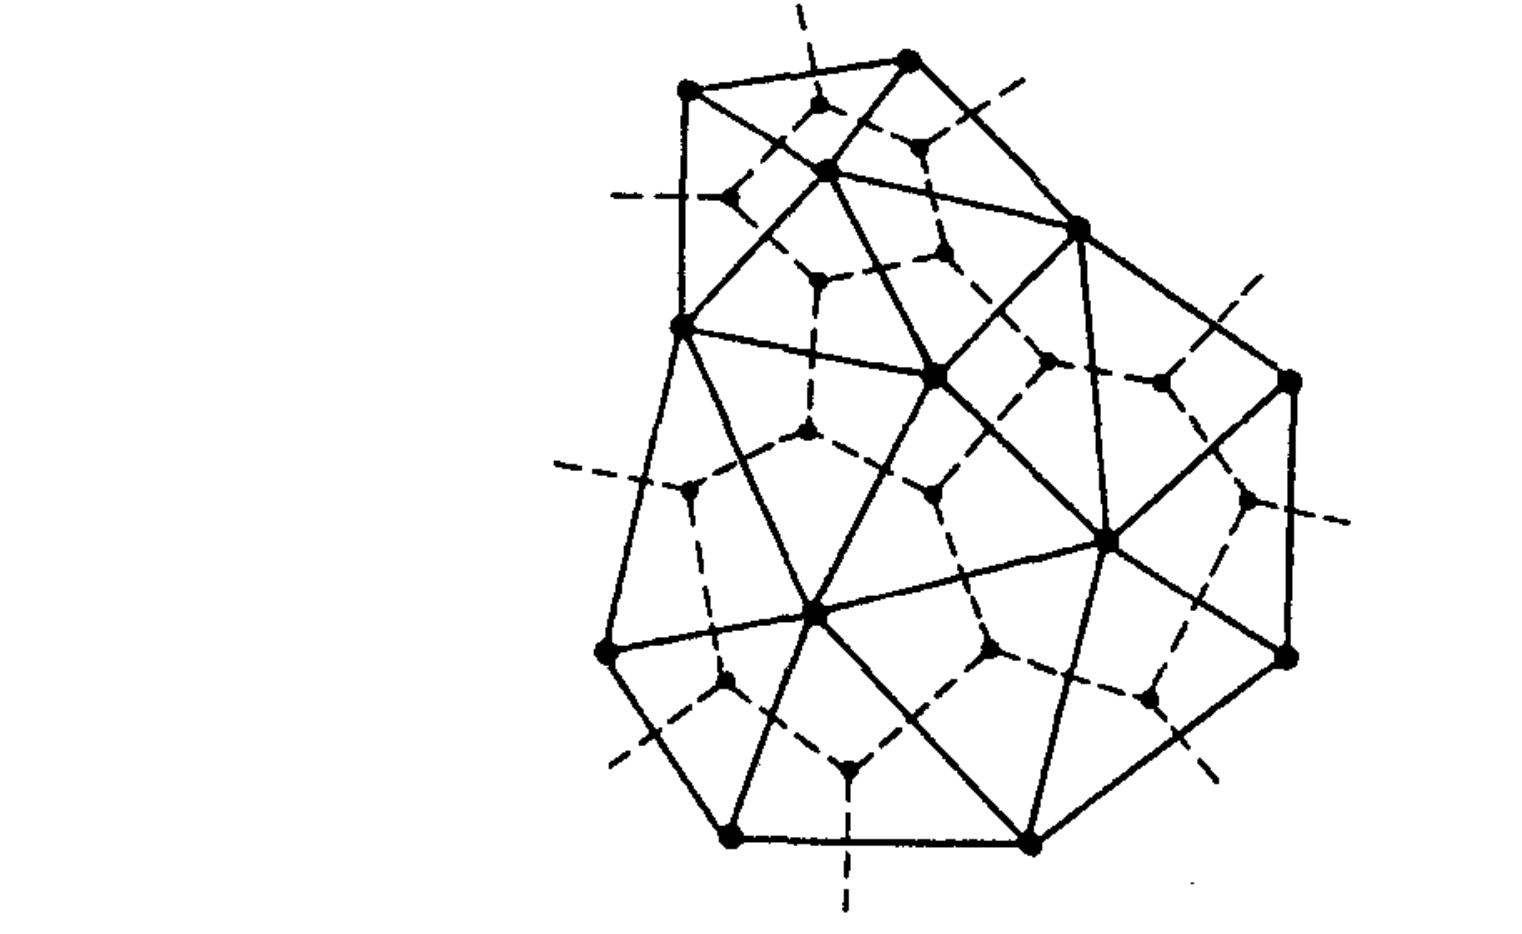
\includegraphics[width=0.46\textwidth]{figures/fig3_6.png}
  \figtitle{3.6}{$m=2$。复形 $K$ 的单形用实线段标出，对偶复形 $DK$ 的单形用虚线段标出}
\end{figure}

现在定义每个单形 $\sigma_{\alpha}^{j}$ 与 $DK$ 的每个多面体 $D\sigma_{\beta}^{j}$ 的\emph{相交指数}（其中 $\sigma_{\alpha}^{j}$ 与 $\sigma_{\beta}^{j}$ 是 $K$ 的同一维数的单形）：若 $\sigma_{\alpha}^{j}$ 与 $D\sigma_{\beta}^{j}$ 相交则取 $1$，否则取 $0$：
\begin{equation}
  \sigma_{\alpha}^{j}\circ D\sigma_{\beta}^{j}=\delta_{\alpha\beta}. \tag{2.33}
\end{equation}
按线性性推广，便得到互补维数的任意一对闭链的\emph{相交指数}：
\begin{gather}
  \Bigl(\sum_{\alpha}\lambda^{\alpha}\sigma_{\alpha}^{j}\Bigr)
  \circ\Bigl(\sum_{\beta}\mu^{\beta}D\sigma_{\beta}^{j}\Bigr)
  =\delta_{\alpha\beta}\lambda^{\alpha}\mu^{\beta},\notag\\
  c\circ Dc'=\delta_{\alpha\beta}\lambda^{\alpha}\mu^{\beta} \tag{2.34}
\end{gather}
（其中右端使用了 Einstein 求和约定）。

在可定向情形，边缘算子与对偶在下述意义下交换：
\begin{equation}
  D\partial(c)=\partial^*D(c). \tag{2.35}
\end{equation}
（对不可定向的 PL 流形，只要系数取自 $\Z/2$，此式仍然成立。）Poincaré 对偶同构 (2.31) 现在可由 (2.35) 推出：给定流形 $M^m$ 的同调，一方面与它的单纯重分 $K$ 的同调一致，另一方面又与把 $M^m$ 重分为凸多面体的 $DK$ 的同调一致。

% CHUNK ch03b DONE
